\section{概述}

\subsection{完成情况}

\subsection{Titanix 介绍}

\subsection{操作系统整体架构}

\begin{figure}[hbt]
    \centering
    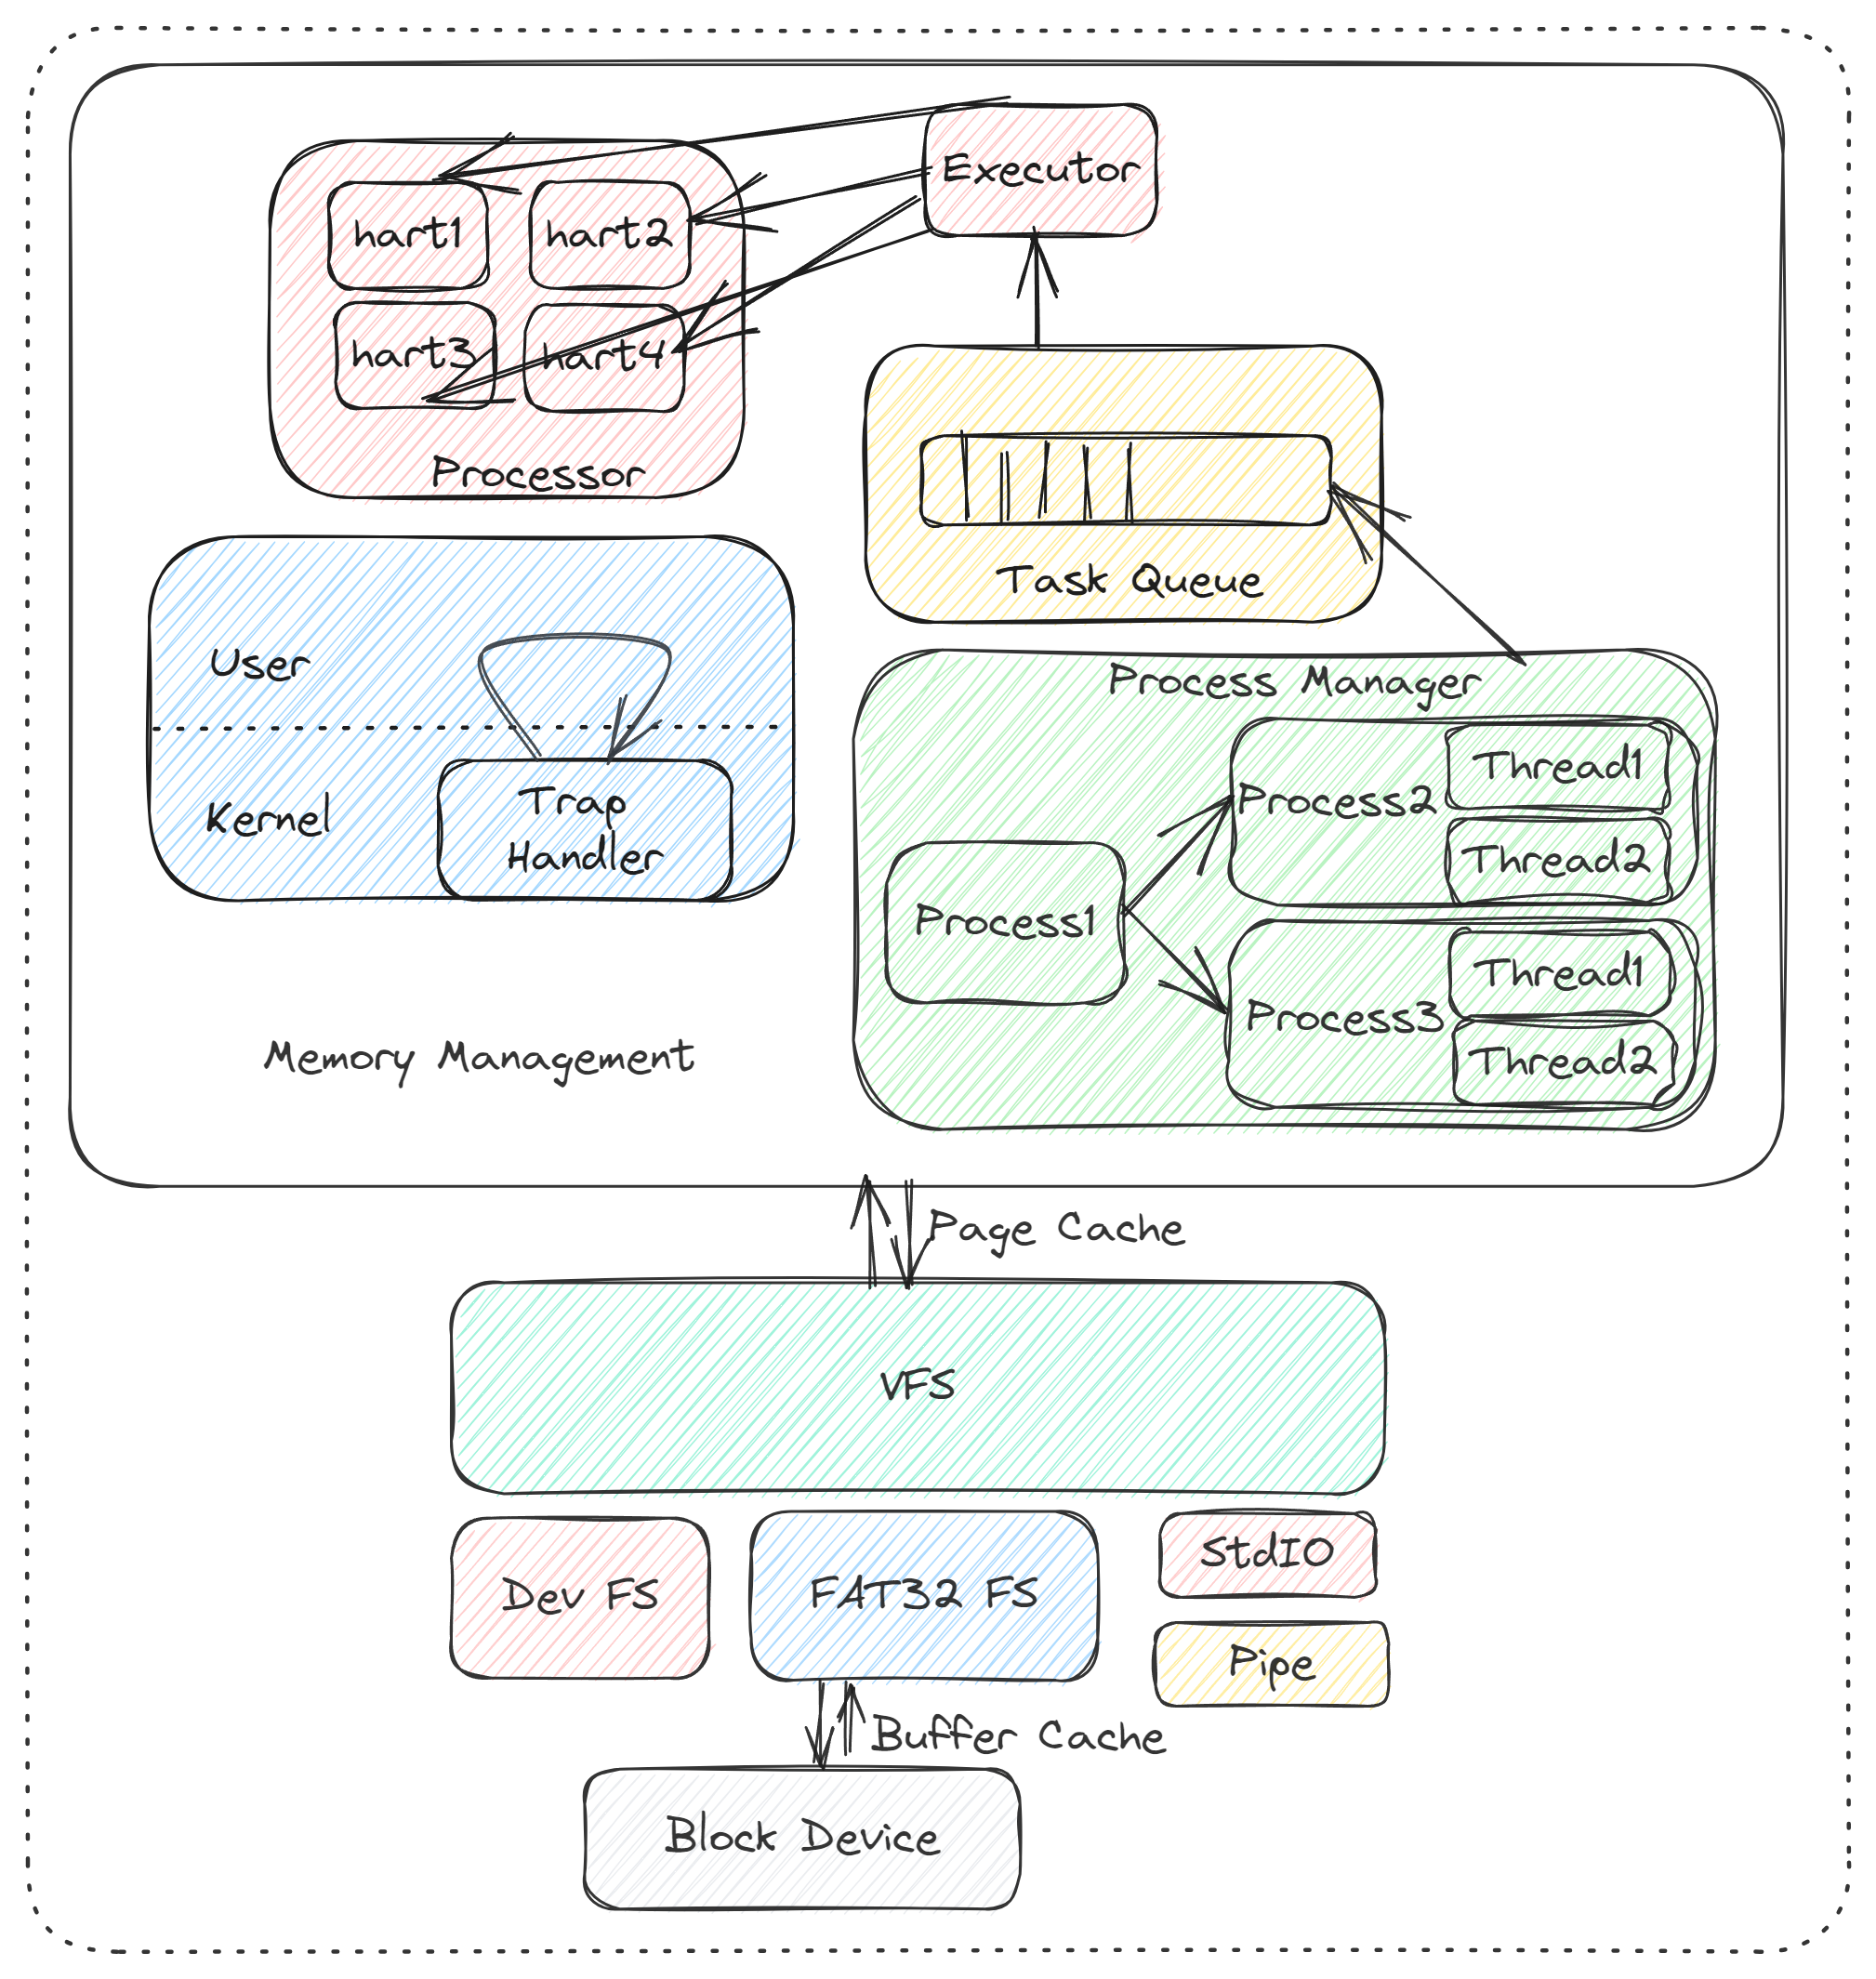
\includegraphics[width=.9\linewidth]{figure/architecture.png}
    \caption{总体架构}
    \label{pic:architecture}
\end{figure}

\subsection{目录和文件描述}

\begin{tcolorbox}[
title=\textbf{os目录树},
listing only,
breakable
]
\begin{minted}[breaklines, baselinestretch=1, fontsize=\small]{text}
|   build.rs
|   gdbinit
|   Makefile
|   tmp.sh
\---src
    |   console.rs
    |   entry.S
    |   lang_items.rs
    |   linker64.ld
    |   loader.rs
    |   main.rs
    |   sbi.rs
    |   timer.rs
    +---boards
    |       mod.rs
    |       qemu.rs
    +---config
    |       board.rs
    |       fs.rs
    |       mm.rs
    |       mod.rs
    |       process.rs
    |       processor.rs
    |       signal.rs
    +---driver
    |   |   mod.rs
    |   \---block
    |           buffer_cache.rs
    |           io_device.rs
    |           mod.rs
    |           sdcard.rs
    |           spi.rs
    |           virtio_blk.rs
    +---executor
    |       mod.rs
    +---fs
    |   |   dirent.rs
    |   |   fd_table.rs
    |   |   file.rs
    |   |   file_system.rs
    |   |   hash_name.rs
    |   |   inode.rs
    |   |   inode_tmp.rs
    |   |   kstat.rs
    |   |   mod.rs
    |   |   pipe.rs
    |   |   stdio.rs
    |   |   uio.rs
    |   |   utsname.rs
    |   +---devfs
    |   |       block_device.rs
    |   |       mod.rs
    |   |       null.rs
    |   |       zero.rs
    |   +---fat32
    |   |       mod.rs
    |   +---fat32_tmp
    |   |       mod.rs
    |   +---procfs
    |   |       mod.rs
    |   \---testfs
    |           mod.rs
    +---mm
    |   |   address.rs
    |   |   frame_allocator.rs
    |   |   heap_allocator.rs
    |   |   mod.rs
    |   |   page.rs
    |   |   page_cache.rs
    |   |   page_table.rs
    |   |   radix_tree.rs
    |   |   recycle_allocator.rs
    |   +---memory_set
    |   |       mod.rs
    |   |       page_fault_handler.rs
    |   |       vm_area.rs
    |   \---user_check
    |           check.S
    |           mod.rs
    +---process
    |   |   manager.rs
    |   |   mod.rs
    |   |   pid.rs
    |   |   _aux.rs
    |   \---thread
    |           exit.rs
    |           mod.rs
    |           schedule.rs
    |           threadloop.rs
    |           thread_resource.rs
    |           thread_state.rs
    |           tid.rs
    +---processor
    |       context.rs
    |       env.rs
    |       hart.rs
    |       mod.rs
    +---signal
    |       mod.rs
    |       signal_context.rs
    |       signal_handler.rs
    +---sync
    |   |   cond_var.rs
    |   |   mod.rs
    |   |   
    |   \---mutex
    |           mod.rs
    |           sleep_mutex.rs
    |           spin_mutex.rs
    +---syscall
    |       dev.rs
    |       fs.rs
    |       mm.rs
    |       mod.rs
    |       process.rs
    |       signal.rs
    |       sync.rs
    +---trap
    |       context.rs
    |       mod.rs
    |       trap.S
    \---utils
        |   error.rs
        |   hash_table.rs
        |   logging.rs
        |   mem.rs
        |   mod.rs
        |   path.rs
        |   string.rs
        \---debug
                mod.rs
                stack_tracker.rs
\end{minted}
\end{tcolorbox}

\subsection{文档相关}

TODO